\chapter{Building Simulation Programs}
\label{cha:building-simulation-programs}

\section{Overview}

As it was already mentioned, an {\opp} model physically consists of
the following parts:

\begin{itemize}
  \item{NED language\index{ned!files} topology description(s). These
      are files with the \ttt{.ned} extension.}
  \item{Message definitions\index{message definitions}, in files
      with \ttt{.msg} extension.}
  \item{Simple modules implementations and other C++ code, in \ttt{.cc}
        files (or \ttt{.cpp}, on Windows)}
\end{itemize}


To build an executable simulation program,
you first need to translate the MSG files\index{msg!files}
into C++, using the message compiler (\ttt{opp\_msgc}).
After this step, the process is the same as building any C/C++
program from source: all C++ sources need to be compiled into object files
(\ttt{.o} files (using gcc on Mac, Linux) or mingw on Windows), or \ttt{.obj} (using MSVC on Windows)),
and all object files need to be linked with the necessary libraries to get
an executable or shared library.

\begin{note}
Compiling NED files directly to C++ classes is no longer supported in
{\opp} 4.0. NED files are always dynamically loaded.
\end{note}

File names for libraries differ for Unix/Linux and for Windows,
and also different for static and shared libraries.
Let us suppose you have a library called Tkenv.
If you are compiling with gcc or mingw, the file name for the static library
would be something like \ttt{libopptkenv[d].a},
and the shared library would be called \ttt{libopptkenv[d].so}.
(libopptkenvd.so would be used for the debug version while libopptkenv.so
is for the release build.) The Windows version of the static library would
be \ttt{libopptkenv.a}, and the DLL would be named \ttt{libopptkenv.dll}.

\begin{note}
With MSVC, the corresponding filenames will be \ttt{opptkenv.lib} and \ttt{opptkenv.dll}.
On Mac OS X, shared libraries have the \ttt{.dylib} extension instead of \ttt{.so}.
\end{note}

In {\opp} 4.0 we recommend to use shared libraries whenever it is possible.
You'll need to link with the following libraries:

\begin{itemize}
  \item{The simulation kernel and class library\index{simulation!kernel},
    called \textit{oppsim} (file \ttt{liboppsim.[so|dll|dylib]} etc).}
  \item{User interfaces. The common part of all user interfaces is
    the \textit{oppenvir} library (file \texttt{liboppenvir.[so|dll|dylib]}, etc),
    and the specific user interfaces are \textit{opptkenv} and \textit{oppcmdenv}
    (\ttt{libopptkenv.[so|dll|dylib]}, \ttt{liboppcmdenv.[so|dll|dylib]}, etc).
    You have to link with \textit{oppenvir}, plus \textit{opptkenv} or
    \textit{oppcmdenv} or both.}
\end{itemize}

Luckily, you do not have to worry about the above details, because
automatic tools like \ttt{opp\_makemake} will take care of the hard
part for you.

The following figure gives an overview of the process of building
and running simulation programs.

\begin{figure}[htbp]
  \begin{center}
%%XXX    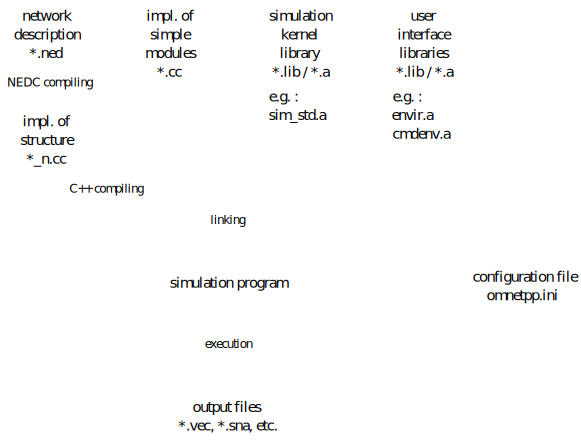
\includegraphics[width=5.992in, height=4.519in]{figures/build}
    \includegraphics{figures/workflow}
    \caption{Building and running simulation}
  \end{center}
\end{figure}


This section discusses how to use the simulation system on the
following platforms:
\begin{itemize}
  \item{Unix (Linux/Mac OS X) with gcc}
  \item{Windows with the included MinGW}
\end{itemize}


\section{Using gcc}

This section applies to using {\opp} on Linux, Solaris, Mac OS X, FreeBSD and
other Unix derivatives, and also to MinGW on Windows.

\begin{note}
The \ttt{doc/} directory of your {\opp} installation contains
\ttt{Readme.}\textit{<platform>} files that provide more detailed platform specific instructions.
\end{note}


\subsection{The opp\_makemake tool}

The \fprog{opp\_makemake} tool can automatically generate a
\texttt{Makefile} for your simulation program, based on the source files
in the current directory or directory tree.
\fprog{opp\_makemake} has several options; \ttt{opp\_makemake -h}
displays help.

The most important options are:

TBD

\subsection{Basic use}

Once you have the source files (\ttt{*.ned}, \ttt{*.msg}, \ttt{*.cc},
\ttt{*.h}) in a directory, change there and type:

\begin{verbatim}
$ opp_makemake
\end{verbatim}

This will create a file named \ttt{Makefile}\index{Makefile}. If you
type \fprog{make}, your simulation program should build.

If you already had a \ttt{Makefile} in that directory, \fprog{opp\_makemake}
will refuse to overwrite it. You can force overwriting the old \ttt{Makefile}
with the -f option:

\begin{verbatim}
$ opp_makemake -f
\end{verbatim}

The name of the output file\index{output!file} will be derived from
the name of the project directory (see later). You can override it
with the \ttt{-o} option:

\begin{verbatim}
$ opp_makemake -f -o aloha
\end{verbatim}

In addition to default target that builds the simulation executable,
the \ttt{Makefile} also contains the following targets:

\begin{longtable}{|l|p{8cm}|}
\hline
\tabheadcol
\tbf{Target} & \tbf{Action}\\\hline
all & The default target is to build the simulation executable\\\hline
depend & Adds (or refreshes) dependencies in the \ttt{Makefile}\\\hline
clean &  Deletes all files that were produced by the make process\\\hline
\end{longtable}


\subsection{Debug and release builds}

todo some text

\begin{verbatim}
$ make MODE=debug
\end{verbatim}

\begin{verbatim}
$ make MODE=release
\end{verbatim}


\subsection{Using external C/C++ libraries}

include directories with -I

linking with external libraries with -l and -L

To define an external library to be linked with, use \ttt{-Ldir} to specify
external library directory and \ttt{-llibrary} to specify the name of the
external dependecy.


\subsection{Building directory trees}

It is possible to build a whole source directory tree with a single makefile.
Each source tree will generate a single output file (executable or library).
A source directory tree will always have a \ttt{Makefile} in its root,
and source files may be placed anywhere in the tree.

To turns on this option, use the \ttt{opp\_makemake --deep} option.
\ttt{opp\_makemake} will collect all \ttt{.cc} and \ttt{.msg} files from
the whole subdirectory tree, and generate a makefile that covers all.
If you need to exclude a specific directory, use the \ttt{-X exclude/dir/path}
option. (Multiple \ttt{-X} options are accepted.)

An example:

\begin{verbatim}
$ opp_makemake -f --deep -X experimental -X obsolete
\end{verbatim}


\subsection{Automatic include dirs}

If your source tree contains several subdirectories (maybe several levels
deep), it is annoying that you should specify relative paths for your
header files in your \ttt{.cc} files or you should specify the include path
explicitly by the \ttt{-I includepath} option. \ttt{opp\_makemake} has a
default automatic include path discovery mechanism, which adds all necessary include
directories in the current source tree to the compiler command line.
Automatic include directories are turned on by default.

\begin{note}
You may turn off the include autodiscovery mechanism with the
\ttt{--no-deep-includes} option.
\end{note}

The only requirement is that your \ttt{\#include} statements must unambigously
specify the name of the header file. (i.e. if you have two \ttt{common.h}
files one in subdir1 and the other in subdir2 specify \ttt{\#include
"subdir1/common.h"} instead of \ttt{\#include "common.h"}. If you want to
include a directory which is outside of your source directory tree you
always must specify it with the \ttt{-I external/include/dir} option.


\subsection{Dependency handling}

TODO what are dependencies

\fprog{opp\_makemake} automatically adds dependencies to the makefile\index{Makefile!dependencies}.
You can regenerate the dependencies by typing \fprog[make]{make depend} any time.
The warnings during the dependency generation process can
be safely ignored.


\subsection{Out-of-directory build}

describe where object files, executables etc are created

The output directory is under the \ttt{out} subdir of the project directory.

\begin{note}
The project directory is the first ancestor of the current directory which
contains a \ttt{.project} file).
\end{note}

The location of the generated output file is determned by the -O option.
(The default value is 'out', relative to the project root directory):

\begin{verbatim}
$ opp_makemake -O ../tmp/obj
\end{verbatim}



\subsection{Building shared and static libraries}

By default the makefile will create an executable file, but it is also
possible to build shared or static libraries. Shared libraries
are usually a better choice.

Use \ttt{--make-so} to create shared libraries, and \ttt{--make-lib}
to build static libraries. The \ttt{--nolink} option completely avoids
the linking step, which is useful for top-level makefiles that only invoke
other makefiles, or if you want to do the linking manually.

TODO: dlls with msvc (export/import symbols like INET\_API)


\subsection{Recursive builds}

The \ttt{--recurse} option enables recursive make: when you build the simulation, make
will descend into the subdirectories and runs make in them too.
By default, \ttt{--recurse} decends into all subdirectories; the -X directory option
can be used to make it ignore certain subdirectories. This option is especially useful
for top level makefiles.

The \ttt{--recurse} option automatically discovers subdirectories, but this
is sometimes inconvenient. With the \ttt{-d dir} or \ttt{--subdir dir} option,
you can explicitly specify which directories to recurse into, and also,
the directories need not be direct children of the current directory.

\begin{note}
With \ttt{--d}, it is also possible to create infinite recursions.
\fprog{opp\_makemake} cannot detect them, it is your responsibility that
cycles do not occur.
\end{note}

The recursive make options (\ttt{--recurse}, \ttt{-d}, \ttt{--subdir})
imply \ttt{-X}, that is, the directories recursed into will be
automatically excluded from deep makefiles.

You can control the order of traversal by adding dependencies into
the \ttt{makefrag} file (see \ref{sec:makefrag})

Motivation for recursive builds:
 - toplevel makefile
 - integrating sources that have their own makefile


TODO revise:

Your source directory tree may contain parts which need their own hand
written \ttt{Makefile}. This can happen if you include source files from an
other non {\opp} project. To include this handwritten \ttt{Makefile} into
the build proecess first exclude that part of the source tree from the deep
file discovery by using the \ttt{-X project/with/own/makefile} and use the
\ttt{--subdir project/with/own/makefile} option to instruct
\ttt{opp\_makemake} to call the handwritten \ttt{Makefile} directly.


\subsection{Customizing the Makefile}
\label{sec:makefrag}

It is possible to add rules or otherwise customize the generated makefile
by providing a \ttt{makefrag} file. When you run \fprog{opp\_makemake}, it
will automatically insert \ttt{makefrag} into the resulting \ttt{Makefile}.
With the \ttt{-i} option, you can also name other files to be included into the
\ttt{Makefile}.

makefrag will be inserted after the definitions but before the first
rule, so it is possible to override existing definitions and add new
ones, and also to override the default target.

Makefrag can be useful if some of your source files are generated
from other files (for example, you use generated NED files), or ....
or ...


\subsection{Projects with multiple source trees}

In the case of a large project, your source files may be spread across
several directories and your project may generate more than one executable
file (i.e. several shared libraries, examples etc.).

Once you have created your makefiles with \ttt{opp\_makemake} in
every source directory tree, you will need a toplevel makefile.
The toplevel makefile usually calls only the makefiles
recursively in the source directory trees.


\subsection{A multi-directory example}

For a complex example of using opp\_makemake, we will check how to create
the makefiles for the mobility-framework. First take a look at the
project's directory structure and find the directories that should be used as
source trees:

\begin{verbatim}
mobility-framework
    bitmaps
    contrib <-- source tree (build libmfcontrib.so from this dir)
    core <-- source tree (build libmfcore.so from this dir)
    docs
    network
    template
    testSuite <-- source tree (build testSuite executable from this dir)
\end{verbatim}

Additionally there are dependencies between these output files: \ttt{mfcontrib}
requires \ttt{mfcore} and \ttt{testSuite} requires both \ttt{mfcore}
and \ttt{mfcontrib}.

First create the makefile for the core directory (build a shared lib from all .cc files
found in the core subtree and name it 'mfcore'):

\begin{verbatim}
$ cd core && opp_makemake -f --deep --make-so -o mfcore -O out
\end{verbatim}

The contrib directory is depending on \ttt{mfcore} so we use the -L and -l options
to specify the library we should link with. Note that we must also add
the include directories manually from the core source tree, because autodiscovery works only
in the same source tree:

\begin{verbatim}
$ cd contrib && opp_makemake -f --deep --make-so -o mfcontrib -O out -I../core/basicModules -I../core/utils -L../out/$(CONFIGNAME)/core -lmfcore
\end{verbatim}

The testSuite will be created as an executable file which depends on both
\ttt{mfcontrib} and \ttt{mfcore}.

\begin{verbatim}
$ cd testSuite && opp_makemake -f --deep -o testSuite -O out -I../core/utils -I../core/basicModules \\
    -I../contrib/utils  -I../contrib/applLayer -L../out/$(CONFIGNAME)/contrib -lmfcontrib
\end{verbatim}

Now the last step is to create a top-level makefile in the root of the project that
calls the previously created makefiles in the correct order. We will use the
--nolink option, exclude every subdirectory from the bild (-X.) and explicitly call
the above makefiles (-d dirname).

\begin{verbatim}
$ opp_makemake -f --nolink -O out -d testSuite -d core -d contrib -X.
\end{verbatim}

Finally we have to specify the dependencies between the above directories. Add the lines below to the makefrag file
in the project directory root.

\begin{verbatim}
contrib_dir: core_dir
testSuite_dir: contrib_dir
\end{verbatim}

\ifcommercial
\section{Using Windows and Microsoft Visual C++}

There are only slight differences to the way Microsoft Visual C++
is handled. The main differences are:
\begin{itemize}
  \item{You should use \ttt{opp\_nmakemake} instead of \ttt{opp\_makemake}}
  \item{The generated makefile will be called \ttt{Makefile.vc} by default.}
  \item{Use \ttt{makefrag.vc} instead of \ttt{makefrag}.}
  \item{\ttt{nmake} is used instead of \ttt{make}.}
  \item{The build process is started by \ttt{nmake -f Makefile.vc} instead of \ttt{make}.}
\end{itemize}

Required compiler settings: turn on exception handling and RTTI, and
set stack size to as low as 64K.
\fi

%%% Local Variables:
%%% mode: latex
%%% TeX-master: "usman"
%%% End:
